% Source: graduate-coursework/Research/Papers/drafts/temporal_context_motion_trails/Radar_TemporalContext_MotionTrails.tex
% Description: Concept overview: echo trails inject a bounded temporal memory into a single-frame input pipeline.

\documentclass[border=4pt]{standalone}
\usepackage{algpseudocode}
\usepackage{amsmath,amssymb}
\usepackage[T1]{fontenc}
\usepackage{pgfplots}
\usepackage{tikz}
\usepackage{xcolor}
\pgfplotsset{compat=1.18}
\usetikzlibrary{arrows.meta,positioning,calc,fit,shapes.geometric,shapes.misc,decorations.pathmorphing,backgrounds}


\newcommand{\ph}[1]{\textcolor{red}{#1}}

\begin{document}
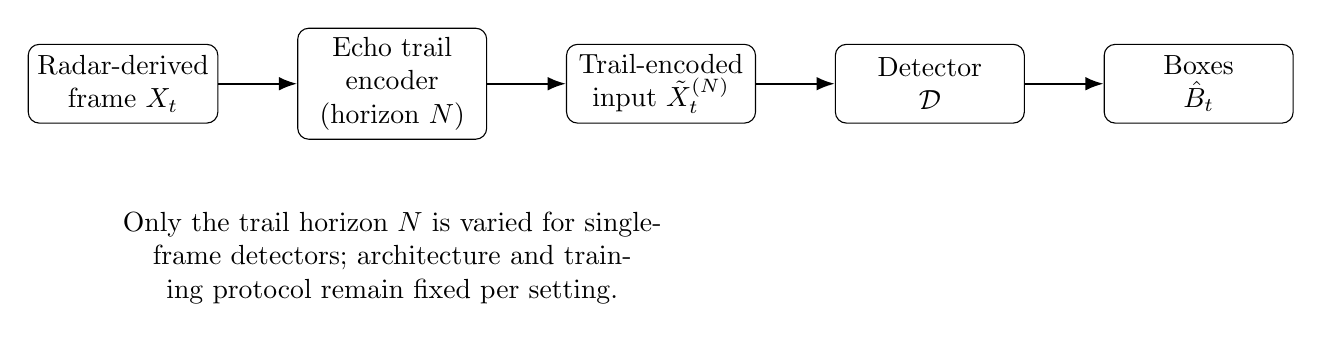
\begin{tikzpicture}[
  node distance=10mm,
  box/.style={draw, rounded corners, align=center, minimum width=24mm, minimum height=10mm},
  arrow/.style={-Latex, thick}
]
\node[box] (raw) {Radar-derived\\frame $X_t$};
\node[box, right=of raw] (trail) {Echo trail\\encoder\\(horizon $N$)};
\node[box, right=of trail] (inp) {Trail-encoded\\input $\tilde{X}_t^{(N)}$};
\node[box, right=of inp] (det) {Detector\\$\mathcal{D}$};
\node[box, right=of det] (out) {Boxes\\$\hat{B}_t$};

\draw[arrow] (raw) -- (trail);
\draw[arrow] (trail) -- (inp);
\draw[arrow] (inp) -- (det);
\draw[arrow] (det) -- (out);

\node[align=center, below=8mm of trail, text width=90mm]
{Only the trail horizon $N$ is varied for single-frame detectors; architecture and training protocol remain fixed per setting.};

\end{tikzpicture}
\end{document}
